My current work concerns the role of information in unsupervised learning, including recent work on contrastive learning \cite{chen2020simple}. I have shown that lower bounds developed for use in experimental design can be usefully applied as objectives in contrastive representation learning. In related work, I would like to undertake a more thorough study of mutual information and entropy gradient estimators. Within experimental design, I am currently working on planning adaptive experiments. There is an important connection to Bayesian reinforcement learning \cite{zintgraf2019varibad}.


\section{Contrastive Learning with Adapted Negatives}
\textit{Expected completion: September 2020} \\
\textbf{Abstract} We introduce Contrastive Learning with Adapted Negatives (CLAN). Unlike InfoNCE and other contrastive objectives, CLAN samples negative examples adaptively in order to pose a more challenging self-supervised learning problem, thereby achieving higher sample-efficiency and learning more informative representations. We present an algorithm that efficiently samples adapted negatives from a cache, then reweights them to more strongly penalize the most serious errors, which results in a new objective function that is a lower bound on mutual information. We show that CLAN can outperform existing methods based on InfoNCE, even with small batch sizes.

\subsection{Introduction}
Unsupervised representation learning holds the key to lowering the sample complexity of deep learning algorithms, and as such remains a key challenge for artificial intelligence.
In order to be useful in subsequent tasks, \textit{good} representations should be low-dimensional and should preserve useful structural information about the potentially high-dimensional inputs.
For example, humans construct abstract linguistic representations of complex perceptual data, which then can be used to make a range of decisions about a scenario.
This is similar to deep learning in that an encoder has to distinguish salient features of the data, which can be useful for tasks that are not known a priori, and can include object detection or segmentation \cite{he2019momentum}, translation \cite{devlin2018bert}, or other tasks \cite{oord2018representation}.

%Unsupervised representation learning remains a key challenge for artificial intelligence.
%Good representations efficiently encode high dimensional data, preserving useful high-level information. These representations can be used in subsequent tasks in place of the original data.
%Humans construct linguistic representations of data which can then be used to make a range of decisions about a scenario. 
%Deep neural networks, when used for unsupervised representation learning, encode high dimensional data to a low dimensional representation which is then used for downstream tasks such as classification. The encoder must learn which features of the data are salient and which can be discarded without knowing which task the features will then be used for.

Many representation learning algorithms can be characterized by a prediction task and an objective function.
The prediction task often involves partitioning data examples into \textit{right-hand} and \textit{left-hand} parts and predicting one from the other or a relation between them.
These left and right parts may be present and future states of a system \cite{oord2018representation}, different modalities of an image \cite{tian2019contrastive}, unmasked and masked words in a sentence \cite{devlin2018bert}, etc.
The objective function, which quantifies the performance and allows training of the model, is often based on predictive likelihood or on contrasting a given data example with a set of negative ones.
This general approach has shown tremendous promise in learning representations that transfer well to downstream tasks \cite{devlin2018bert,henaff2019data}.


%What objective function should we use to train such an encoder network? Self-supervised learning creates an objective function for unsupervised representation learning by hiding the `right-hand' part of the input data and trying to predict it from the `left-hand' part. These `left' and `right' parts may in fact be present and future states of a system \cite{oord2018representation}, different modalities of an image \cite{tian2019contrastive}, unmasked and masked words in sentence \cite{devlin2018bert}, etc. This general approach has shown tremendous promise in learning representations that transfer well to downstream tasks \cite{devlin2018bert,henaff2019data}.


% [CMC is actually using a variant of InfoNCE]
Many self-supervised techniques use the InfoNCE objective \cite{oord2018representation,tian2019contrastive,hjelm2018learning}, which sets up a classification problem: given the encoding of the left-hand input, choose the corresponding right-hand from $K$ possibilities including the true sample, and $K-1$ negative samples chosen uniformly at random from the rest of the dataset. 
In expectation, this objective function is a lower bound on the mutual information between the representation of the left and right parts of the input.

Choosing the negative samples uniformly at random may result in a classification task that is not particularly difficult---we see this mathematically from the fact that InfoNCE cannot exceed $\log K$ \cite{poole2019variational} and empirically from the fact that large minibatches are typically required for these methods to perform well \cite{henaff2019data,ozair2019wasserstein}.

The contributions of this paper are threefold. 
Firstly, we propose an algorithm that encourages representations to contain more fine-grained information about the right-hand target by posing a more challenging classification task.
This is inspired by `hard example mining' \cite{shrivastava2016training} and accomplished by choosing the negative samples in an adaptive fashion based on the given left-hand input.
%
%Firstly, we propose an algorithm that allows choosing the negative samples in an adaptive fashion based on the given left-hand input. 
%This poses a more challenging classification task, which will encourage representations to contain more fine-grained information about the right-hand target, inspired by `hard example mining' \cite{shrivastava2016training}.
%We must do this in a computationally efficient manner without re-encoding the entire dataset at every iteration. 

Secondly, we introduce a computationally efficient manner of adaptive negative sampling, where we avoid recomputing representations of the whole dataset.
This is achieved by storing previously encountered inputs and their representations in a multi-layer cache, which then allows us to sample negatives proportional to how likely they are to fool the $K$-way classifier.
This is similar to stochastic variational memory addressing \cite{bornschein2017vma}.
%This can be viewed as applying (stochastic) hard attention \cite{vaswani2017attention} over the cache. 

%Secondly, our proposed algorithm allows us to obtain negatives samples from a multi-layer \textit{cache} and avoids recomputing representations on the cache. We sample negatives proportional to how likely they are to fool the $K$-way classifier. This can be viewed as applying (stochastic) hard attention \cite{vaswani2017attention} over the cache. 

Finally, we should give a lesser penalty for mistakenly choosing a difficult negative sample---one that is a plausible if incorrect completion of the left-hand input---and a greater penalty for choosing something completely wrong.
Our third key idea is that by \textit{reweighting} the negative samples we can correctly penalize easy and difficult negatives.
With the correct reweighting, we obtain a new objective function for self-supervised learning that uses adapted negatives but is still a lower bound on mutual information which can be larger than $\log K$.
The resulting algorithm, CLAN can learn highly informative representations with a batch size of 8.
We expect the benefits of this approach to be most apparent on complex tasks that require more fine-grained information.

\subsection{Background}


A number of recent works have reported state-of-the-art representation learning results using self-supervision with the InfoNCE objective.
Contrastive Predictive Coding (CPC) attempts to predict a future state $z_{t+k}$ from an aggregation of past states $c_t = A(z_1, ..., z_t)$ \cite{oord2018representation}. 
By considering an image as an ordered sequence of patches, CPC has also been applied to image classification \cite{henaff2019data}. 
Deep Infomax (DIM) is closely-related to image-based CPC but it leverages local patch and global image encodings as opposed to ordered patch sequences \cite{hjelm2018learning}.
In Contrastive Multi-view Coding (CMC), we attempt to predict image modalities from each other; the modalities include the \textit{L} and \textit{ab} channels in case of pure image datasets, but also segmentation masks and depth images if these are available \cite{tian2019contrastive}. 
In each of the approaches, datapoints are split into parts: past-future, local-global and \textit{L-ab}.
We abstract this modelling choice by considering a dataset of left-right pairs.

%We formalize this by considering a dataset of abstract left-right pairs $(\x_i, \y_i)_{i=1}^N$ with representations $\bu_i = \bu(\x_i)$ and $\bv_i = \bv(\y_i)$.


Given a dataset of left-right pairs $(\x_i, \y_i)_{i=1}^N$, we encode them to obtain representations $\bu_i = \bu(\x_i)$ and $\bv_i = \bv(\y_i)$. 
%The left-right distinction is an abstraction: in CPC as originally formulated \cite{oord2018representation} the pairs are an aggregation of past states, and the future state; CPC and Deep Infomax (DIM) \cite{hjelm2018learning} used different patches of a single image; in CMC the pairs are different modalities of a whole image e.g. the \textit{L} and \textit{ab} channels.
The classification task posed by InfoNCE is: given a left-hand input $\bu_1$, choose the correct right-hand pair $\bv_1$ from $K$ possibilities comprising the true sample $\bv_1$ and $K-1$ negative samples $\bv_2, ..., \bv_K$.
The negative samples are typically other samples in the same minibatch as $\bu_1$, which means that they are chosen uniformly at random from the dataset and independently of $(\bu_1, \bv_1)$.
The $K$-way classification is done by a critic $f \ge 0$, where $f(\bu, \bv)~=~\exp(\bu^T\bv)$ is a common choice. The InfoNCE objective is closely-related to the cross-entropy, and for a single positive example $\bu_i$ reads as
\begin{equation}
\mathcal{L}_\text{InfoNCE}(\bu_1,\bv_{1:K}) = \log  \frac{f(\bu_1, \bv_1)}{\frac{1}{K}\sum_{k=1}^K f(\bu_1, \bv_k)}\,.
\end{equation}
It is typically averaged over a minibatch of positive examples $\bu_{1:K}$.
%when summed over a mini-batch $(\bu_i,\bv_i)_{i=1}^K$ this gives
%\begin{equation}
%	\mathcal{L}_\text{InfoNCE}(\bu_{1:K},\bv_{1:K}) = \frac{1}{K}\sum_{k=1}^K \log \frac{f(\bu_k, \bv_k)}{\frac{1}{K}\sum_{\ell=1}^K f(\bu_k, \bv_\ell)}
%\end{equation}

Now, to discuss the connection to mutual information, we take a probabilistic perspective.
%To discuss the connection to mutual information, we take a probabilistic perspective.
The matching pair of samples $\bu_1, \bv_1 \sim p(\bu, \bv)$ comes from the \textit{joint} distribution over left-right pairs, while the negatives $\bv_2, ..., \bv_K \iid p(\bv)$ are sampled independently from the \textit{marginal}.
This amounts to the probabilistic version of choosing uniformly at random from the dataset.
The mutual information between $\bu$ and $\bv$ describes how much knowing $\bu$ tells us about $\bv$; formally it is given by
\begin{equation}
I(\bu,\bv) = \E_{p(\bu,\bv)}\left[ \log \frac{p(\bu, \bv)}{p(\bu)\,p(\bv)} \right].
\end{equation}


In expectation over $p(\bu_1,\bv_1)\,p(\bv_{2:K})$, the InfoNCE objective is a lower bound on mutual information \cite{poole2019variational}, i.e.
\begin{equation}
I(\bu,\bv) \ge \E_{p(\bu_1,\bv_1)\,p(\bv_{2:K})}[\mathcal{L}_\textsc{infonce}].
\end{equation}
Thus maximizing $\mathcal{L}_\textsc{infonce}$ by stochastic gradient amounts to maximizing a lower bound on the mutual information between representations of the left- and right-hand parts of the data.

For small minibatches the classification task solved by InfoNCE may be relatively easy.
This is expressed mathematically by the fact that, since $f\ge 0$, $\mathcal{L}_\text{InfoNCE}$ is itself upper bounded,
\begin{equation}
\mathcal{L}_\textsc{infonce} \le \log \frac{f(\bu_1,\bv_1)}{\frac{1}{K} f(\bu_1, \bv_1)} = \log K.
\end{equation}
This upper bound means that, unless the batch size is large, InfoNCE-driven encoders will struggle to improve once this information capacity is reached.

\subsection{Method}
%\subsection{Sampling adapted negatives}
%\label{sec:method:sampling}

%In order to learn informative representations of data without supervision we must learn to extract salient features of an object by considering it \textit{in relation to} itself and other objects in the dataset. InfoNCE achieves this by considering left and right parts of one object, and comparing these to corresponding parts of other objects in the dataset. It forms a $K$-way classification problem: given $\bu_1$ pick out the positive sample $\bv_1$ against a background of $K-1$ negatives $\bv_{2:K}$ chosen uniformly at random from the dataset. This is guaranteed to increase the information that $\bu$ carries about its completion $\bv$. However, the information will only increase up to a point. Once the $K$-way classification can be solved well, representations are no longer encouraged to extract further information from the underlying data.

%What if we were to choose negative samples that already look like a good match for $\bu_1$? Initially, negative samples may match the positive sample on the few basic features that have already been extracted by the encoder. The harder classification task then encourages the encoder to pick out more fine-grained features in order to select the positive sample correctly. This in turn leads us to pose a more challenging classification task.

%Alternatively, instead of considering large sets of negative samples, one  could draw the negative samples from a distribution conditional on the positive sample $\bu_1$, that is $\bv_2, ..., \bv_K \iid q(\bv \mid \bu_1)$.
%To achieve this, we propose drawing negative samples from a distribution conditional on $\bu_1$, i.e. $\bv_2, ..., \bv_K \iid q(\bv \mid \bu_1)$.
%This allows us to adapt the negative samples to match $\bu_1$, but avoids deterministically selecting negatives which may lead to overfitting, and ensures we occasionally include very different objects as negatives.
%More specifically, one could sample the negatives from a distribution proportional to the critic, i.e.\  $q(\bv \mid \bu_1) \propto f(\bu_1, \bv)$.
%That is, we choose samples proportionally to how much the critic $f$ already thinks they are a good match for $\bu_1$.
%However, this naive idea is clearly computationally infeasible because it requires computing the representations $\bv(\y_i)$ and evaluating $f(\bu_1, \bv_i)$ for the whole dataset $i=1,...,N$. % Having done this, we might as well use \textit{all} $\bv_{2:N}$ as negative samples. [this could be shorter / more concise]

Contrastive representation learning works by learning to distinguish between data samples.
In InfoNCE this amounts to a $K$-way classification problem;
once this classification problem is solved well for the majority of minibatches drawn from the data, there is no incentive to further improve the representations.
This motivates the use of large batch sizes \cite{henaff2019data} and memory banks \cite{he2019momentum,tian2019contrastive,wu2018unsupervised} to store previously seen data samples---both methods allow increasing the size of negative sample sets and lead to more difficult classification problems, but have high memory costs and suffer from performance issues as stored representations become stale.

Instead, we propose a method of choosing negative examples in an adaptive fashion, which allows dispensing with large sets of negative samples.
More specifically, it is possible to choose hard negative samples by sampling from a distribution conditional on $\bu_i$, that is $\bv_2, ..., \bv_K \iid q(\bv \mid \bu_1)$.

More specifically, one could sample the negatives from an empirical distribution proportional to the critic scores, i.e.\  $q(\bv~\mid~\bu_1)~\propto~f(\bu_1,~\bv)$, which results in negative samples that are maximally similar to the considered positive example under the current critic.
%That is, we choose samples proportionally to how much the critic $f$ already thinks they are a good match for $\bu_1$.
This approach is computationally infeasible, however, as it requires recomputing the representations $\bv(\y_i)$ and evaluating the critic $f(\bu_1, \bv_i)$ for the whole dataset $i=1,...,N$.

We reduce the computational load associated with finding negative examples by \textit{caching} representations encountered in previous training iterations.
We then sample negatives $\bv$ from $q(\bv \mid \bu_1) \propto f(\bu_1, \bv^\text{cache})$ using the cached representations.
This is similar to \cite{he2019momentum,wu2018unsupervised}, with the difference that we sample a small number of $K-1$ negatives from this distribution and recompute the representations of the chosen negatives.
This approach affords the benefits of a large cache---we are able to find challenging negatives to provide a strong learning signal---whilst still using up-to-date representations in the objective to allow correct gradients to flow to the encoder.
%There is a clear link between our approach and hard attention [citation]: we use cached representations to select a small number of items in the cache to attend to, and then compute the corresponding up-to-date representations for those items which will enter into the objective.
Figure~\ref{fig:clan_data_flow} depicts our approach.

\begin{table}[t]
	\caption{Computational cost of different operations to evaluate the InfoNCE and CLAN objectives on one minibatchbatch. $B$ is the batch size, $C$ is the cache size, $K - 1$ is the number of negatives; for InfoNCE, $B=K$ and elements in the mini-batch are re-used as negative examples.}
	\label{tab:complexity}
	\begin{center}
		\begin{small}
			\begin{tabular}{lcc}
				\toprule
				&  InfoNCE & CLAN  \\
				\midrule
				Disk reads & $\mathcal{O}(B)$ & $\mathcal{O}(B)$   \\
				Computing negative distribution & - & $\mathcal{O}(BC)$ \\
				Encoder forward passes & $\mathcal{O}(B)$ & $\mathcal{O}(BK)$       \\
				Critic evaluations & $\mathcal{O}(BK)$ & $\mathcal{O}(BK)$ \\
				\bottomrule
			\end{tabular}
		\end{small}
	\end{center}
	\vskip -.16in
\end{table}

\begin{figure*}[t]
	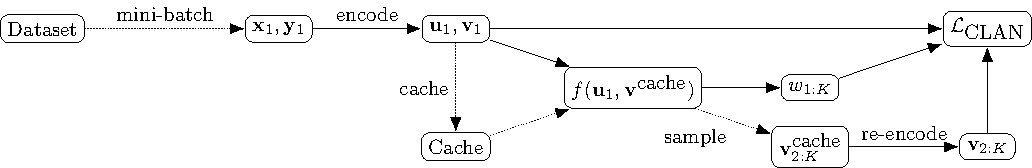
\includegraphics[width=.95\textwidth]{figures/data_flow.pdf}
	\caption{Outline of CLAN. Data points are encoded, and the encodings cached. Negative samples $\bv_{2:K}$ are sampled from the distribution $q(\bv \mid \bu_1) \propto f(\bu_1, \bv^{\text{cache}})$, re-encoded, and weighted by $p(\bv_i)/q(\bv_i\mid\bu_1)$. Positive and negative samples, and weights are combined to evaluate the objective. Solid lines represent operations that backpropagate gradients; dotted lines are detached from the autograd computational graph.}
	\label{fig:clan_data_flow}
\end{figure*}

For large datasets, we maintain a cache of size $C << N$ of  the most recently seen representations $(\bu^\text{cache}_i, \bv^\text{cache}_i)_{i=1}^C$ and additionally a cache of the original datapoints $(\x_i,\y_i)_{i=1}^C$.
Caching the original datapoints is essential to prevent additional disk reads when recomputing embeddings of the negative samples.
%We found that this caching technique leads to runtime speed that approaches that of InfoNCE-based methods (CPC, CMC) but provides a much stronger learning signal.
%Table~\ref{tab:complexity} shows the computational cost of our approach as compared to InfoNCE on a minibatch of size $B$ (which may now be varied independently of $K$).
In practice, the caches were implemented as first-in-first-out queues, meaning they comprised the $C$ most recently encoded points. Table~\ref{tab:complexity} shows the computational cost of our approach as compared to InfoNCE on a minibatch of size $B$ (which may now be varied independently of $K$).



% We can then compute fresh representations to evaluate the actual objective, ensuring the correct gradients flow to the encoder. This approach can work well for moderate datasets and may be seen as applying hard attention across the entire dataset to choose adapted negatives. Scanning the entire dataset is infeasible when $N$ is very large. In this case, we maintain a cache of size $C$ of the most recently seen samples and sample $\bv$ using the same sampling distribution restricted to the cache.  [this paragraph needs further development]
%
%In our approach, we have decoupled the batch size $B$ from the number of negative samples $K-1$. Table~\ref{tab:complexity} summarizes the computational complexity of our approach compared to InfoNCE.
%
%[todo: should we include this? Is the BC term correct or should it be BC + BCK or BC + BK log C ....] In practice the sampling is fast so, if $B=K$, both are $K^2$.


%\begin{table}[t]
%	\caption{Computational cost of different operations to evaluate the InfoNCE and CLAN objectives on one minibatchbatch. $B$ is the batch size, $C$ is the cache size, $K - 1$ is the number of negatives; for InfoNCE, $B=K$ and elements in the mini-batch are re-used as negative examples.}
%	\label{tab:complexity}
%	\begin{center}
%		\begin{small}
%			\begin{tabular}{lcc}
%				\toprule
%				& InfoNCE & CLAN  \\
%				\midrule
%				Disk reads & $\mathcal{O}(B)$ & $\mathcal{O}(B)$   \\
%				Computing negative distribution & - & $\mathcal{O}(BC)$ \\
%				Encoder forward passes & $\mathcal{O}(B)$ & $\mathcal{O}(BK)$       \\
%				Critic evaluations & $\mathcal{O}(BK)$ & $\mathcal{O}(BK)$ \\
%				\bottomrule
%			\end{tabular}
%		\end{small}
%	\end{center}
%	\vskip -.16in
%\end{table}


\paragraph{Reweighting Adapted Negatives}
%We have devised a method to sample negatives that are likely to pose a more challenging classification task than if we simply chose negatives uniformly at random from the dataset, specifically negatives are now sampled from a distribution $q(\bv\mid\bu_1)$. Using these adapted negatives in the InfoNCE objective is inappropriate for several reasons. Under an InfoNCE loss, the penalty for misclassification is the same for every negative. For example, if the encoder matches the left-hand image of a dog with the right-hand image of a similar but different dog, the InfoNCE penalty is the same as when it matches this left-hand image with the right-hand image of a car. More formally, we have changed the sampling distribution from $p(\bu_1, \bv_1)p(\bv_{2:K})$ to $p(\bu_1, \bv_1)q(\bv_{2:K}\mid\bu_1)$ meaning that $\E_{p(\bu_1, \bv_1)q(\bv_{2:K}\mid\bu_1)}[\mathcal{L}_\text{InfoNCE}(\bu_1, \bv_{1:K})]$ will no longer be a lower bound on mutual information $I(\bu, \bv)$.

The adapted negatives are likely to pose a more challenging classification task than if we simply chose negatives uniformly at random from the dataset.
However, using the adapted negatives in the InfoNCE objective corresponds formally to changing the sampling distribution from $p(\bu_1, \bv_1)p(\bv_{2:K})$ to $p(\bu_1, \bv_1)q(\bv_{2:K}\mid\bu_1)$, which then means that the resulting objective will no longer be a lower bound on mutual information.

%Using the adapted negatives in the InfoNCE objective leads to several issues, however.
%Firstly, under an InfoNCE loss, the penalty for misclassification is the same for every negative.
%For example, if the encoder matches the left-hand image of a dog with the right-hand image of a similar but different dog, the InfoNCE penalty is the same as when it matches this left-hand image with the right-hand image of a car.
%More formally, we have changed the sampling distribution from $p(\bu_1, \bv_1)p(\bv_{2:K})$ to $p(\bu_1, \bv_1)q(\bv_{2:K}\mid\bu_1)$ meaning that $\E_{p(\bu_1, \bv_1)q(\bv_{2:K}\mid\bu_1)}[\mathcal{L}_\text{InfoNCE}(\bu_1, \bv_{1:K})]$ will no longer be a lower bound on mutual information $I(\bu, \bv)$.

Restricted to the cache of size $C$, $q(\bv\mid\bu_1)$ is a categorical distribution over $C$ items and $p(\bv) = 1/C$ is the original uniform distribution over the same items.
Our proposal is to reweight the negative samples using importance weights
\begin{equation}
w_i = \frac{p(\bv_i)}{q(\bv_i\mid\bu_1)}
\end{equation}
as in importance sampling \cite{kahn1953methods}. 
%Importance weights have the defining property that they preserve the expectation under a change in distribution:
%\begin{equation}
%	\E_{q(\bv_i\mid \bu_1)}[w_ih(\bv_i)] = \E_{p(\bv_i)}[h(\bv_i)]
%\end{equation}
%where $h$ is any measurable function.
%
%
%We see that $w_i$ is large when $q(\bv_1\mid\bu_1)$ is small, i.e. we upweight samples which look like a poor match for $\bu_1$ such as the right-hand of a car when compared against the left-hand of a dog. 
%
%
%The $p(\bv_i)$ term here corresponds to the original sampling scheme which is uniformly at random over the dataset, hence $p(\bv_i) = 1/N$. (This is true when $q$ is supported on the dataset, see Appendix X for the case using a cache.)
Specifically, we propose the following CLAN objective
\begin{equation}
\label{eq:clan}
\mathcal{L}_\textsc{CLAN}(\bu_1,\bv_{1:K}) = \log \frac{f(\bu_1, \bv_1)}{\frac{1}{K}\sum_{k=1}^K w_k f(\bu_1, \bv_k)}.
\end{equation}
This loss is illustrated in Figure~\ref{fig:diagram:clan}.
The `penalty' for the critic assigning a high value to $\bv_k$ for $k>1$ is now $w_k f(\bu_1, \bv_k)$. The weight $w_k$ is large when $q(\bv_k\mid\bu_1)$ is small, so we upweight the penalty for samples which look like a poor match for $\bu_1$ such as the right-hand of a car when compared against the left-hand of a dog. Applied to a mini-batch $(\x_i,\y_i)_{i=1}^B$, the CLAN objective is
\begin{equation}
\label{eq:clan_batch}
\mathcal{L}_\textsc{CLAN}^\text{batch} = \frac{1}{B}\sum_{i=1}^B \log \frac{f(\bu_i, \bv_i)}{\frac{1}{K}\sum_{k=1}^K w_{ik} f(\bu_i, \bv_{ik})}
\end{equation}
where $\bv_{i1} = \bv_i$,  $\bv_{ik}\iid q(\bv\mid \bu_i)$ for $k=2,...,K$ and $w_{ik} = p(\bv_{ik}) / q(\bv_{ik}\mid \bu_i)$.


\begin{figure*}[t]
	\centering
	\begin{subfigure}[t]{0.45\textwidth}
		\centering
		\vskip 0pt
		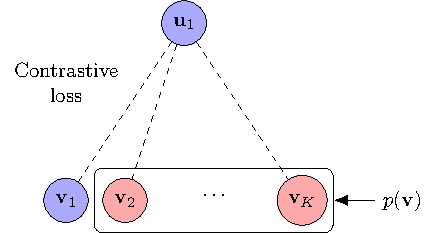
\includegraphics[scale=1]{figures/infonce_diagram.pdf}
		\vspace{10pt}
		\caption{InfoNCE \label{fig:diagram:infonce}}
	\end{subfigure}
	~
	\begin{subfigure}[t]{0.45\textwidth}
		\centering
		\vskip 0pt
		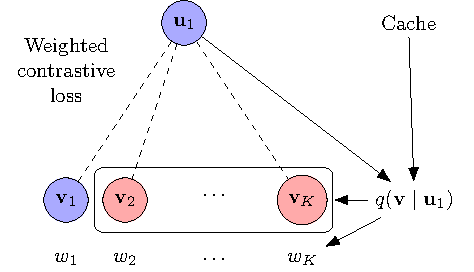
\includegraphics[scale=1]{figures/clan_diagram.pdf}
		\caption{CLAN \label{fig:diagram:clan}}
	\end{subfigure}
	\caption{An illustration of the contrastive learning problems posed by (a) InfoNCE, and (b) CLAN. }
	\vspace{-5pt}
	\label{fig:diagrams}
\end{figure*}


The precise choice of reweighting in equation~\eqref{eq:clan} has the important consequence that the CLAN objective is a lower bound on the mutual information under the \textit{new} sampling distribution $p(\bu_1, \bv_1)q(\bv_{2:K}\mid \bu_1)$, i.e.
\begin{equation}
\label{eq:clan_lb}
I(\bu,\bv) \ge \E_{p(\bu_1, \bv_1)q(\bv_{2:K}\mid \bu_1)}[\mathcal{L}_\textsc{CLAN}(\bu_1,\bv_{1:K})].
\end{equation}
This inequality follows from a connection between $\mathcal{L}_\textsc{CLAN}$ and a recently proposed mutual information estimator for the expected information gain in experimental design \cite{foster2019unified}. By linearity of the expectation, $\mathcal{L}_\textsc{CLAN}^\text{batch}$ is also an information lower bound. 
% The bound \eqref{eq:clan_lb} holds for any choice of adapted negative distribution $q(\bv\mid\bu_1)$, so exotic methods of sampling negatives will still lead to valid lower bounds when the correct reweighting is applied. 

In practice, we applied our method both with and without reweighting, and found that empirically reweighing was important to give the best performance.

Unlike $\mathcal{L}_\textsc{INFONCE}$, $\mathcal{L}_\text{CLAN}$ is not bounded above by $\log K$ allowing the encoder to learn representations that are highly informative about the target even when the number of negatives is small. For the sampling scheme outlined in this section with a cache of size $C$, we can upper bound the CLAN objective
\begin{align}
\mathcal{L}_\textsc{CLAN} & \le \log \frac{f(\bu_1, \bv_1)}{\frac{1}{K}w_1 f(\bu_1,\bv_1)} \\
&= \log \frac{K}{\left(\frac{1/C}{q(\bv_1\mid \bu_1)}\right)} \\
& \le \log(CK).
\end{align}
We see that CLAN has the bottleneckm of InfoNCE with batch size of $CK$ whilst only requiring $K-1$ negative samples.

Overall, $\mathcal{L}_\textsc{CLAN}$ is new objective for self-supervised methods including CPC and CMC that is a lower bound on mutual information. It chooses \textit{adapted} negative samples to ensure that the encoder faces an increasingly difficult classification task and so continues to learn more fine-grained features present in the data. CLAN uses a reweighting to penalize the most serious misclassifications more. The resulting objective provides a stronger learning signal for the encoder enabling it to learn more informative representations. We can see this mathematically from the fact that, unlike InfoNCE, the new objective can exceed $\log K$.

\subsection{Proofs}
For completeness, we include the proof that $\mathcal{L}_\text{CLAN}(\bu_1, \bv_{1:K})$ is an information lower. We need to prove the following inequality
\begin{equation}
	\E_{p(\bu,\bv)}\left[\log \frac{p(\bu,\bv)}{p(\bu)p(\bv)} \right] \ge \E_{p(\bu_1,\bv_1)q(\bv_{2:K})}\left[\log \frac{f(\bu_1,\bv_1)}{\frac{1}{K}\sum_{i=1}^K \frac{p(\bv_i)f(\bu_1,\bv_i)}{q(\bv_i|\bu_1)}} \right]
\end{equation}
We first show that 
\begin{equation}
	\int \frac{p(\bu_1)p(\bv_1)q(\bv_{2:K}|\bu_1)f(\bu_1,\bv_1)}{\frac{1}{K}\sum_{i=1}^K \frac{p(\bv_i)f(\bu_1,\bv_i)}{q(\bv_i|\bu_1)}} \ d\bu_1\,d\bv_{1:K} = 1
\end{equation}
We have
\begin{align}
\int \frac{p(\bu_1)p(\bv_1)q(\bv_{2:K}|\bu_1)f(\bu_1,\bv_1)}{\frac{1}{K}\sum_{i=1}^K \frac{p(\bv_i)f(\bu_1,\bv_i)}{q(\bv_i|\bu_1)}} \ d\bu_1\,d\bv_{1:K} &= \E_{p(\bu_1)p(\bv_1)q(\bv_{1:K}|\bu_1)}\left[ \frac{f(\bu_1,\bv_1)}{\frac{1}{K}\sum_{i=1}^K \frac{p(\bv_i)f(\bu_1,\bv_i)}{q(\bv_i|\bu_1)}} \right] \\
&= \E_{p(\bu_1)q(\bv_{2:K}|\bu_1)}\left[ \frac{\frac{p(\bv_1)f(\bu_1,\bv_1)}{q(\bv_1|\bu_1)}}{\frac{1}{K}\sum_{i=1}^K \frac{p(\bv_i)f(\bu_1,\bv_i)}{q(\bv_i|\bu_1)}} \right]
\end{align}
Now we note that in the last line, $\bv_{1:K}$ are exchangeable. That means any expectation under $q(\bv_{1:K})$ is unchanged if we permute the indices $1, ..., K$. Hence for $j \in \left\{1, ..., K \right\}$ we have
\begin{equation}
	\int \frac{p(\bu_1)p(\bv_1)q(\bv_{2:K}|\bu_1)f(\bu_1,\bv_1)}{\frac{1}{K}\sum_{i=1}^K \frac{p(\bv_i)f(\bu_1,\bv_i)}{q(\bv_i|\bu_1)}} \ d\bu_1\,d\bv_{1:K} = \E_{p(\bu_1)q(\bv_{2:K}|\bu_1)}\left[ \frac{\frac{p(\bv_j)f(\bu_1,\bv_j)}{q(\bv_j|\bu_1)}}{\frac{1}{K}\sum_{i=1}^K \frac{p(\bv_i)f(\bu_1,\bv_i)}{q(\bv_i|\bu_1)}} \right]
\end{equation}
Finally, by linearity of the expectation, we may take the mean over $j$ to see that
\begin{align}
\int \frac{p(\bu_1)p(\bv_1)q(\bv_{2:K}|\bu_1)f(\bu_1,\bv_1)}{\frac{1}{K}\sum_{i=1}^K \frac{p(\bv_i)f(\bu_1,\bv_i)}{q(\bv_i|\bu_1)}} \ d\bu_1\,d\bv_{1:K} &= \frac{1}{K}\sum_{j=1}^K\E_{p(\bu_1)q(\bv_{2:K}|\bu_1)}\left[ \frac{\frac{p(\bv_j)f(\bu_1,\bv_j)}{q(\bv_j|\bu_1)}}{\frac{1}{K}\sum_{i=1}^K \frac{p(\bv_i)f(\bu_1,\bv_i)}{q(\bv_i|\bu_1)}} \right] \\
&=\E_{p(\bu_1)q(\bv_{2:K}|\bu_1)}\left[ \frac{\frac{1}{K}\sum_{j=1}^K\frac{p(\bv_j)f(\bu_1,\bv_j)}{q(\bv_j|\bu_1)}}{\frac{1}{K}\sum_{i=1}^K \frac{p(\bv_i)f(\bu_1,\bv_i)}{q(\bv_i|\bu_1)}} \right] \\
&= 1.
\end{align}
We then have the following
\begin{align}
	\E_{p(\bu_1,\bv_1)}\left[\log \frac{p(\bu_1,\bv_1)}{p(\bu_1)p(\bv_1)} \right] &= \E_{p(\bu_1,\bv_1)q(\bv_{2:K})}\left[\log \frac{p(\bu_1,\bv_1)q(\bv_{2:K}|\bu_1)\frac{f(\bu_1,\bv_1)}{\frac{1}{K}\sum_{i=1}^K \frac{p(\bv_i)f(\bu_1,\bv_i)}{q(\bv_i|\bu_1)}}}{p(\bu_1)p(\bv_1)q(\bv_{2:K}|\bu_1)\frac{f(\bu_1,\bv_1)}{\frac{1}{K}\sum_{i=1}^K \frac{p(\bv_i)f(\bu_1,\bv_i)}{q(\bv_i|\bu_1)}}} \right] \\
	&= \E_{p(\bu_1,\bv_1)q(\bv_{2:K})}\left[\log \frac{f(\bu_1,\bv_1)}{\frac{1}{K}\sum_{i=1}^K \frac{p(\bv_i)f(\bu_1,\bv_i)}{q(\bv_i|\bu_1)}}\right] \\ &\ + KL\left(p(\bu_1,\bv_1)q(\bv_{2:K}|\bu_1) \middle \| \frac{p(\bu_1)p(\bv_1)q(\bv_{2:K}|\bu_1)f(\bu_1,\bv_1)}{\frac{1}{K}\sum_{i=1}^K \frac{p(\bv_i)f(\bu_1,\bv_i)}{q(\bv_i|\bu_1)}} \right) \\
	&\ge \E_{p(\bu_1,\bv_1)q(\bv_{2:K})}\left[\log \frac{f(\bu_1,\bv_1)}{\frac{1}{K}\sum_{i=1}^K \frac{p(\bv_i)f(\bu_1,\bv_i)}{q(\bv_i|\bu_1)}}\right]
\end{align}
We use the first result to write the remainder term as a KL divergence.

\section{Optimal planning of adaptive experiments using Bayesian RL}
\textit{Expected completion: October 2020} \\
\textbf{Abstract} To plan a Bayesian-optimal sequence of adaptive experiments, one needs to conduct inference using the data seen so far, estimate the expected information gain (EIG) of each candidate design for the next step under the current posterior, choose the best design, and use it to conduct the next experiment. Several of these steps are computationally challenging, and for complex models prohibitively so. We propose a framework that \textit{amortizes} the expensive steps in this process. This allows us to train a \textit{design network} that is trained intensively on simulated data, but at deployment time can select an approximately optimal experimental design for the next stage of an experiment using a single forward pass. Our approach proceeds by casting the experimental design process as a Bayes Adaptive Markov Decision Process (BAMDP) with a reward signal driven by the state inference problem. Extending existing methods for Bayesian RL, we show how the design network can be trained to approximate the optimal policy.

\subsection{Casting adaptive experimental design as a BAMDP}
A Bayes Adaptive Markov Decision Process \cite{guez2015sample,zintgraf2019varibad} consists of a state space $\mathcal{S}$, action space $\mathcal{A}$, horizon $H$, reward $R$, transition model $T$ and initial state distribution $T_0$. We also include a hidden state $m$ with prior distribution $p(m)$. The reward and transition functions depend on $m$. Having applied a sequence of actions $a_1, ..., a_t$ resulting in states $s_1, ..., s_t$ and rewards $r_1, ..., r_t$ we form the \textit{belief state} $p_t(m) = p(m|a_{1:t},y_{1:t},r_{1:t})$. The next state is distributed as
\begin{equation}
	s_{t+1} \sim \E_{p_t(m)}[T(s_{t+1}|s_t,a_t,m)]
\end{equation}
and the expected reward is
\begin{equation}
	\E[R_{t+1}] = \E_{p_t(m)T(s_{t+1}|s_t,a_t,m)}[R(a_{1:t}, s_{1:t+1},m)].
\end{equation}
The objective is to maximize the following
\begin{equation}
	\mathcal{J} = \E_{p(m), T_0, T, \pi}\left[ \sum_{t=0}^{H-1} R(s_t,a_t,s_{t+1},m) \right]
\end{equation}
(we ignore the discount factor).

Adaptive experimental design consists of a design space $\Xi$, latent variable $\theta$ with prior $p(\theta)$, observation space $\mathcal{Y}$, and likelihood $p(y|\theta,\xi)$. At time $t$ having conducted experiments with designs $\xi_1, ..., \xi_t$ and observed $y_1, ..., y_t$, we must select $\xi_{t+1}$. The Bayes-optimal design for a sequence of $N$ experiments is the one which maximizes the following
\begin{equation}
	I(\xi_{1:t}) = \E_{p(\theta)\prod_{i=1}^N p(y_i|\theta,\xi_i)}\left[ \log \frac{p(\theta|\xi_{1:N},y_{1:N})}{p(\theta)} \right].
\end{equation}
That the optimal design sequence is the one which leads to the greatest reduction in uncertainty about the latent $\theta$. The connection to BAMDPs can be seen by making the following substitutions
\begin{align}
	\text{State space } \mathcal{S} &\leftrightarrow \text{Observation space } \mathcal{Y} \\
	\text{Action space } \mathcal{A} &\leftrightarrow \text{Design space } \Xi \\
	\text{Horizon } H &\leftrightarrow \text{Sequence length } N \\
	\text{Reward } R(a_{1:t},s_{1:t+1},m) &\leftrightarrow \text{Pointwise information }\log \frac{p(\theta|\xi_{1:t+1},y_{1:t+1})}{p(\theta|\xi_{1:t},y_{1:t})} \\
	\text{Hidden variable } m &\leftrightarrow \text{Latent variable } \theta \\
	\text{Prior } p(m) &\leftrightarrow \text{Prior } p(\theta) \\
	\text{Transition model } T(s_{t+1}|s_t, a_t, m) &\leftrightarrow \text{Likelihood } p(y|\theta,\xi) \\
	\text{Initial state distribution } T_0 &\leftrightarrow \text{No initial observation}
\end{align}
We then have
\begin{align}
	\mathcal{J} &= \E_{p(m), T_0, T, \pi}\left[ \sum_{t=0}^{H-1} R(s_t,a_t,s_{t+1},m) \right] \\
	&= \E_{p(\theta)\prod_{i=1}^N p(y_i|\theta,\xi_i), \pi}\left[ \sum_{t=0}^{N-1} \log \frac{p(\theta|\xi_{1:t+1},y_{1:t+1})}{p(\theta|\xi_{1:t},y_{1:t})} \right] \\
	&= \E_{p(\theta)\prod_{i=1}^N p(y_i|\theta,\xi_i), \pi}\left[  \log \frac{p(\theta|\xi_{1:N},y_{1:N})}{p(\theta)} \right] \\
	&= I(\pi)
\end{align}
the objective for experimental design.

We see that experimental design fits well into the BAMDP setting. However, there are some distinctions to be drawns. In a BAMDP, the reward is an external signal. In experimental design, the reward is defined through Bayesian inference on the latent $\theta$. Computing the reward is typically intractable. We hope to make use of variational estimators \cite{foster2019unified} as a way of estimating the reward and so learning a good design network.

\section{Invariance in representation learning}
\textit{Expected completion: February 2021} \\
\textbf{Abstract} Mutual information has arisen as an important objective in the training of unsupervised representations \cite{oord2018representation}. Expanding the mutual information as $I(\z;\x) = H(\z) - \E_{p(\x)}[H(\z|\x)]$ we interpret the first term as encouraging high \textit{entropy} representations, the second as encouraging \textit{invaraiance} to a range of augmentations and perturbations. This connects mutual information driven learning with existing work on invariance \cite{cohen2019general,lyle2020benefits}. We show that existing methods to encourage invariance including equivariant architecture and feature averaging can further decrease the term $\E_p(\x)[H(\z|\x)]$ and improve downstream utility of the representations.

\section{Gradient estimators for mutual information and entropy}
\textit{Expected completion: February 2021} \\
\textbf{Abstract} A number of recent methods propose to estimate and optimize the mutual information or closely related objectives without using an explicit density model. Starting from the Kraskov estimator \cite{kraskov2004estimating}, we consider more recent objectives based on the Donsker-Varadhan representation \cite{belghazi2018mine}, self-supervised objectives such as InfoNCE \cite{oord2018representation} and Stein estimators \cite{li2017gradient,shi2018spectral}. We compare existing estimators and their implied gradient estimators, showing that many can be connected directly or indirectly to kernel density estimation. We further analyze the bias and variance of these estimators both theoretically and empirically. 


